% Drawing 144/04-6 -- folder 144, batch 04, archive page 68 (PDF page 69).
% Transcription: En bas à gauche, une sphère : un sommet unique au pôle nord, d'où partent plusieurs méridiens, certains en pointillé (la carte cyclotomique à un sommet, une face et $n$ arêtes).
% Kind: sphere: one vertex, meridians (cyclotomic one-vertex map). Method 2 (schematic redraw from the facsimile). Status: ok.
% Notes: Sphere with a single vertex at the north pole; four meridians leave it, two solid and two dotted (back). The mark "o" above the vertex is drawn as a label 0 (reading uncertain).
% Coordinates: 1 unit = 1 mm = 1/100 of the crop width (bbox in page fractions: [0.1, 0.76, 0.28, 0.88]).
% Redrawn by Claude (claude-opus-5-5), issue #73, 2026-11-07; not checked by a human; not compiled (no TeX in the session).
% Rights: reproduces part of the work -- behind RENDER_TRANSCRIPTS, never published by itself.
\documentclass[tikz,border=3pt]{standalone}
\usepackage{amsmath,amssymb}
\usetikzlibrary{patterns,arrows.meta}
\tikzset{pencil/.style={black!45}, struck/.style={black!35}, mark/.style={circle,draw,inner sep=1.3pt}, pt/.style={circle,fill,inner sep=0.9pt}, opt/.style={circle,draw,fill=white,inner sep=1.1pt}}
\begin{document}
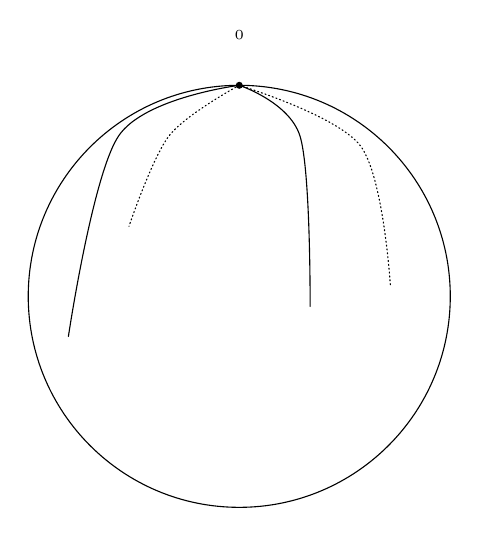
\begin{tikzpicture}[x=1mm,y=1mm,line cap=round,line join=round,font=\scriptsize]
\draw (46.3,-56.2) circle[radius=26.8];
\node[pt] at (46.3,-29.4) {};
\node[inner sep=1pt] at (46.3,-23) {\tiny $0$};
\draw plot[smooth, tension=0.55] coordinates {(46.3,-29.4) (31,-35.8) (24.6,-61.3)};
\draw[densely dotted] plot[smooth, tension=0.55] coordinates {(46.3,-29.4) (37.4,-35.8) (32.3,-47.3)};
\draw plot[smooth, tension=0.55] coordinates {(46.3,-29.4) (54,-35.8) (55.3,-57.5)};
\draw[densely dotted] plot[smooth, tension=0.55] coordinates {(46.3,-29.4) (61.7,-37.1) (65.5,-54.9)};
\end{tikzpicture}
\end{document}
